
%(BEGIN_QUESTION)
% Copyright 2011, Tony R. Kuphaldt, released under the Creative Commons Attribution License (v 1.0)
% This means you may do almost anything with this work of mine, so long as you give me proper credit

Et par motordrevne kompressorer jobber i tandem for å komprimere gass ved et industrielt ammoniakkanlegg:

$$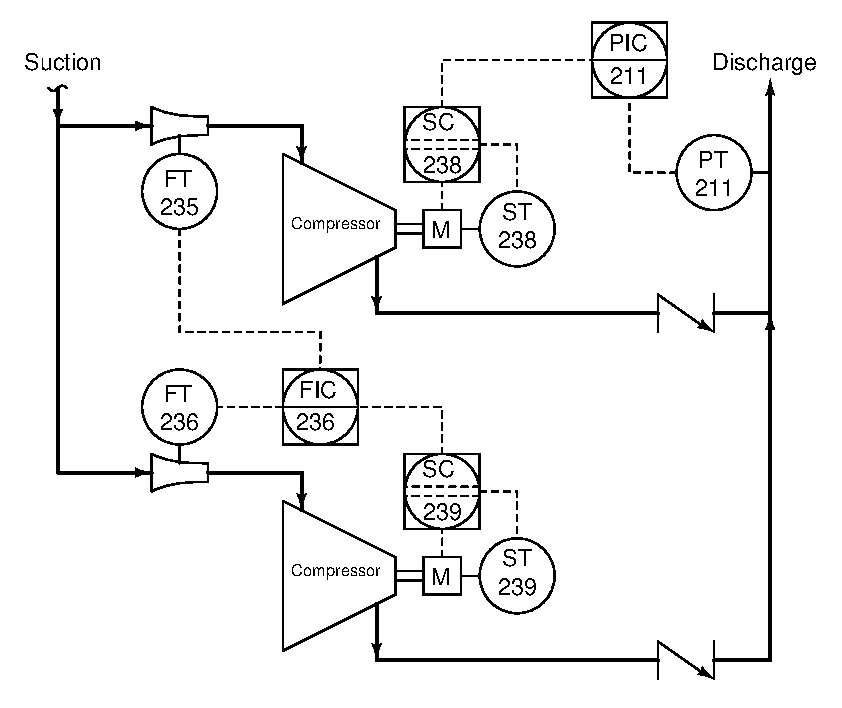
\includegraphics[width=15.5cm]{i00700x01.eps}$$

Forklar hvordan dette reguleringssystemet forsøker å fordele lasten jevnt mellom de to kompressorene, slik at ingen av dem jobber hardere enn den andre, samtidig som begge bidrar til et felles mål.

\vskip 80pt

Forklar i tillegg hva som skjer hvis flowmåler FT-235 feiler med lavt signal.

\vfil

\underbar{file i00700no}
\eject
%(END_QUESTION)





%(BEGIN_ANSWER)

Dette er en vurderingsoppgave -- ingen svar eller hint oppgis!

%(END_ANSWER)





%(BEGIN_NOTES)

Øvre kompressors hastighet er kaskaderegulert av utløpstrykk. Nedre kompressors hastighet er kaskaderegulert av flow. Siden flowraten inn i øvre kompressor brukes som settpunkt for nedre kompressors flowregulator, vil nedre kompressor forsøke å matche flow i 1:1-forhold.

\vskip 10pt

Hvis FT-235 feiler lavt, får nedre kompressors flowregulator fjernsettpunkt lik null. Da stopper den, og all last legges på øvre kompressor. Øvre kompressor øker da hastigheten for å opprettholde utløpstrykket. Nedre tilbakeslagsventil hindrer tilbakestrøm fra øvre kompressors utløp gjennom den stoppede nedre kompressoren.

%INDEX% Regulering, strategier: ratio
%INDEX% Prosess: laststyring av kompressorer

%(END_NOTES)
